\section{Project Description}

\subsection{Our Approach}
Our approach to build a modular set of tools that can be used to convert markdown documents into html and pdf format. These tools will be used to develop a command line interface for markdown parsing.

Our approach has two advantages over other solutions:
\begin{itemize}
	\item Developing our software in c++ will result in a product that is faster than solutions
	\item We will develop an API and release the full source code for the components of our product, allowing other programmers to develop their own tools using our code
\end{itemize}
For example, gimli, made by Fredrik Wallgren is written using Ruby~\cite{gimli}, and md-to-pdf made by Simon Hänisch is written in Javascript~\cite{md-to-pdf}. Gimli and md-to-pdf are both command line tools, but we believe that we can speed them up by using c++.

\subsection{Target Users}

We have two target user groups:
\begin{itemize}
  \item People who want to preview markdown as they work on it. This group will use our command line application to convert between markdown and pdf or html/css.
  \item People who want to develop software that involves parsing or rendering markdown. This group will mix-and-match modules of our software with their own software to take advantage of tools we will build in order to make the command line utility work.
\end{itemize}

\subsection{Interactions}

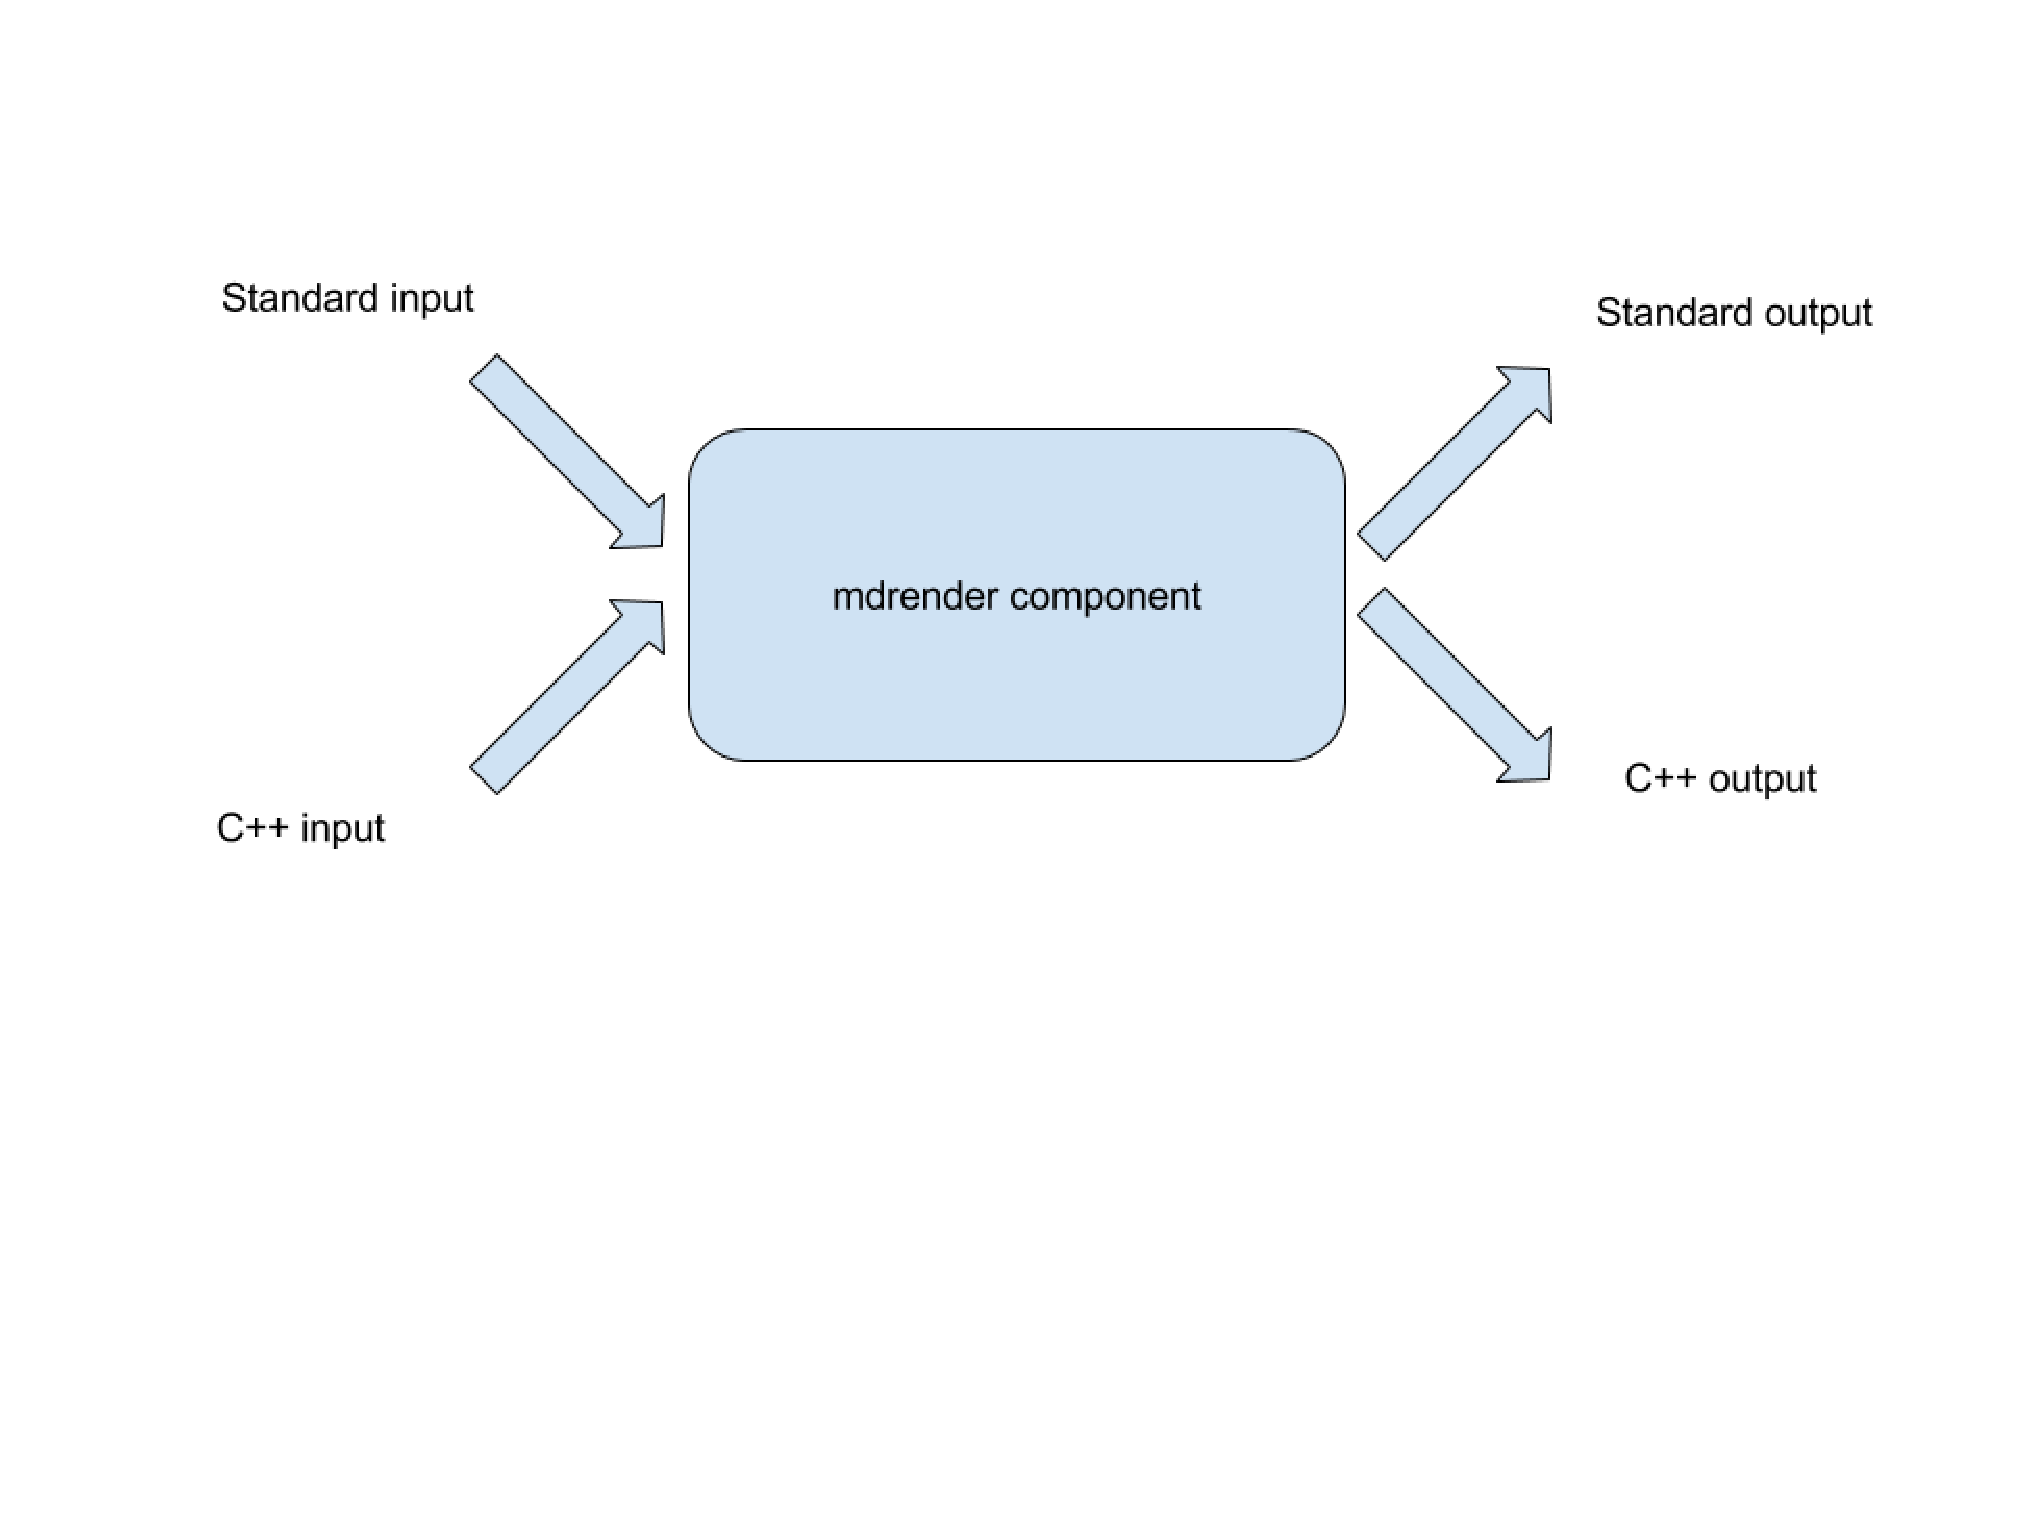
\includegraphics[width=500pt]{images/mdrender_interactions.eps}

This diagram shows how mdrender is designed to be as compatible as possible with other programs by accepting input both via standard in and from other c++ programs as well as outputting data both to standard out and to other c++ programs.

\subsection{Tools}
For this program will be use the following tools and programming languages:
\begin{itemize}
	\item c++ with the g++ compiler
	\item the googletest framework for c++ testing
	\item git and github for source control
\end{itemize}



\subsection{Requirements}

\subsubsection{Functional Requirements}

\begin{itemize}
	\item The system shall be divided into modules that:
		\begin{itemize}
			\item Parse markdown into c++ data
			\item Convert markdown data to pdf data
			\item Convert markdown data to html data
			\item Write pdf and html data to a local file
		\end{itemize}
	\item Each module will be capable of communicating via standard in/out and with other c++ programs
	\item The system will include a command line program that uses all of the modules to convert markdown to pdf or html
\end{itemize}

\subsubsection{Non-functional Requirements}
\begin{itemize}
	\item The system will be optimized to work as quicky as possible
	\item The system will provide a well-documented api to allow others to use the system's functionality
\end{itemize}

\subsection{Documentation}

We will provide comprehensive documentation for both the inner and outer functions of our code.

The main README.md file in the mdrender git repository will provide instructions for installing and using the mdrender command line utility; this will be relatively short, as the program is not complicated.

We will also provide additional README files with each of our modules that will document the public functions for those modules; these will be mirrored by comprehensive code commands for each function. This documentation will give programmers who use our API access to detailed information about how to correctly use the code we create.

\subsection{Features}

\subsubsection{Core Features}

The four core features of our program are:
\begin{itemize}
  \item Parsing markdown files
  \item Converting markdown data to pdf data
  \item Converting markdown data to HTML/CSS data
  \item A command-line utility that encapsulates all of the above features
\end{itemize}

\subsubsection{Additional Features}
Given time, we would also implement these features:
\begin{itemize}
  \item Adding a "listen" or "watch" option to the command line tool that would monitor a markdown file for changes and re-render it every time it changed
  \item Adding the option to select custom styling so that users can use styles other than github flavored markdown
\end{itemize}
